\documentclass[11pt, twoside, a4paper]{article}
\usepackage{epigraph}
\usepackage{graphicx}
\usepackage[swedish]{babel}

\usepackage[margin=3cm]{geometry}
\usepackage{multicol, float, blindtext, kantlipsum}

\usepackage[citestyle=verbose-ibid, bibstyle=authoryear, natbib=true, url=false, doi=false, isbn=false, backend=biber, labeldateparts]{biblatex}
\AtEveryBibitem{%
  \clearlist{language}%
}
%\usepackage{hyperref}
\addbibresource{bibtex/kandidatarbete.bib}

\usepackage{csquotes}

\usepackage{sectsty}
\subsubsectionfont{\normalfont\itshape}
%\subsectionfont{\normalfont\centering}

\usepackage{titlesec}
\titleformat{\section}
  {\normalfont\LARGE\bfseries}{\thesection}{1em}{}[{}]
  % \titlerule[0.8pt]

\title{Värden och värden:\\
	\large en studie av kollektiv sonifiering
}
\author{Karl Johannes Jondell}
\date{\today}

\begin{document}

% \maketitle

% \begin{abstract}
% Vad handlar detta projekt om?
% \end{abstract}

% \begin{keyword}
% sonifiering \sep% 
% diabetes \sep%
% interaktion
% \end{keyword}

\tableofcontents
\clearpage

\newpage
\begin{multicols}{2}

\section*{Introduktion}
\addcontentsline{toc}{section}{Introduktion}
Denna text kompletterar mitt examensprojekt, \emph{[jag behöver komma på ett namn]}, en interaktiv komposition/installation som generarar musik av blodsockervärden. Installationen består av ett SuperCollider-program som skapar själva musiken och en webbplats där man kan lyssna på den, läsa om projektet och ladda upp sina egna blodsockervärden. När en deltagare laddar upp sina värden slussas dessa direkt vidare till SuperCollider-programmet, som i sin tur inkluderar dem i musiken, antingen direkt eller att de blir schemalagda i en kö. Musiken strömmas till webbplatsen (och vidare till lyssnaren) via en internetradiostation. På så sätt utgör musiken ett kontinuerligt flöde som deltagare och åhörare hör samtidigt: det finns ingen början, mitten eller slut, utan endast ett \emph{nu}. Denna förhållning till \emph{temporalitet} utgör ett huvudtema i projektet, jämte med \emph{interaktivitet} (deltagande), \emph{radioteknologi}, \emph{autoimmuna sjukdomar} och \emph{sonifiering}.

% TODO minska antalet "huvudteman"...?!
% TODO "tystnad i radio"
%\emph{(I skrivande stund är installationen inte helt färdig.)}


\subsection*{Bakgrund}
\addcontentsline{toc}{subsection}{Bakgrund}
Idéen om att göra musik av blodsockervärden föddes dagen då jag fick en \emph{Freestyle Libre}-mätare, en så kallad kontinuerlig blodsockermätare (en. \emph{continous glucose monitoring}, eller \emph{CGM}). Denna typ av blodsockermätare skiljer sig från tradionella mätare --- som man är tvungen att sticka sig i fingret och på så sätt mäta blodsockret med --- i att den regelbundet gör mätningar, vilket ger en kontinuerlig kurva över ens blodsockervärden. Kurvorna påminde mig om hur ljudsignaler ofta representeras visuellt (en horisontell tidsaxel och en linjär vertikal axel) och i ett tidigt experiment gjorde jag en direkt översättning av mina blodsockerkurvor till ljudfiler: en så kallad \emph{audifiering} (en. \emph{audification}). Dessa ljud använde jag som samplingar i mitt stycke \emph{Värden och en vagga} (2017), som var ett av arbetsproverna jag sökte till Musikhögskolan med. 

Jag utvecklade vidare och förbättrade mitt första program som jag hade skrivit för att översätta mina kurvor till ljudfiler, så att vem som helst skulle kunna använda programmet och översätta sina enga värden till ljud. Jag byggde också en wavetable-synth i SuperCollider som använde dessa ljudfiler som källmaterial. Detta instrument har jag använt i ett antal olika kompositioner som jag skrivit under min skoltid. Båda dessa program (översättaren och wavetable-synthen) har jag publicerat på min Github\footnote{https://github.com/kj-jondell/Diabetes-Synth}. En del av denna kod återanvände jag även i detta projekt.

%Interaktivitet (\emph{Calling out of context})...

%Radio (\emph{Tuning a radio}, etc...)
%Projekt från ettan, diabetes-synth, radiostation, etc.
%\kant[2-2]
\subsection*{Radio}
\addcontentsline{toc}{subsection}{Radio}
En del av installationen består av en internetradiostation, som strömmar ut den genererade musiken. Just denna ...

Radion som konstmedium har länge inspirerat mig, från hörspelen av bland andra Öyvind Fahlström, till John Cages radiokompositioner, till mer sentida \emph{radioqualia}... 

Hot/cool media (McLuhan), interaktion, "Ring så spelar vi", 
%Digital mediekonst som bygger kring internetradio, eller så kallad \emph{streaming culture}, 
%använder sonifieringar

% \emph{r a d i o q u a l i a}...


\subsection*{Sonifiering}
\addcontentsline{toc}{subsection}{Sonifiering}
%\kant[3-3]
Sonifiering (eller är det verkligen sonifiering). \footcite[2]{bijsterveld_sonic_2019}
Smalley och spektromorfologin. \footnote{Olika ordningar av \emph{surrogacy},  gestaltandet av \emph{datan}.} Bearbetad data och orginaldata. Sensorfel.

\emph{Audification} \footcite[302]{noauthor_sonification_2011} är en form av sonifiering där mätdatan översätts direkt till ljudkurvor... fyra grupper av data (\emph{sound recording}, \emph{general acoustic}, \emph{physical}, och \textbf{\emph{abstract}})...

% \subsubsection*{Det mätbara och det omätbara}
% \addcontentsline{toc}{subsubsection}{\textit{Det mätbara och det omätbara}}
% Bornemark \footcite{bornemark_det_2018}
% Bijsterveld \footcite[100-102]{bijsterveld_sonic_2019}
% McLuhan \footcite[2]{mcluhan_understanding_2015}

\subsection*{Diabetes}
\addcontentsline{toc}{subsection}{Diabetes}
%\kant[4-4]

%\subsubsection*{Communities}
%\addcontentsline{toc}{subsubsection}{\textit{Communities}}

\subsubsection*{Blodsockervärden}
\addcontentsline{toc}{subsubsection}{\textit{Blodsockervärden}}
Blodsocker mäts i mmol/L och varierar hos en icke-diabetiker mellan 4 och 6 mmol/L [källa]. Hos en diabetiker kan detta värde variera från under 1 till över 30 mmol/L, och Freestyle Libre-sensorn har ett spann på att mäta från lägst 2,2 till 27,7 mmol/L (annars visar den \emph{LO} respektive \emph{HI}). Freestyle Libre-sensorn mäter kontinuerligt var 15:e minut.

%Att s.k. \emph{mappa} denna data till musikaliska parametrar är förstås godtyckligt --- värdena i sig har ingen musikalisk mening --- och bör så vara: det är helt enkelt mina konstnärliga val som bestämmer hur de förhåller sig till varandra. Även en bearbetad signal går att använda för att styra musiken: interpolation (mellan de diskreta mätpunkterna), variation (FFT, derivator, etc.), stokastiska egenskaper (auto-korrelation etc), statistiska egenskaper (median, medel, etc.). ''\emph{Tid i målområdet}'' och liknande värden kan också vara intressanta att använda, och har medicinsk betydelse.

%Det som är viktigt i denna \emph{mappning} är dock att den gestaltade datan --- dvs. musiken --- \textbf{inte} får avslöja något om den underliggande eller bakomliggande (mät)datan. Dels är det en integritetsfråga, som diskuteras vidare nedan, dels är det en förutsättning för detta projekt: det existerar inga \emph{bra} eller \emph{dåliga} värden. Själva delningen av värdena är det viktiga.

\subsubsection*{Förhållandet till mätandet}
\addcontentsline{toc}{subsubsection}{\textit{Förhållandet till mätandet}}
I sin text \emph{Det autoimmuna jaget --- om att sätta gränser} \footcite[286]{arvidson_det_2016} skriver Mats Arvidson om kravet som diabetiker på disciplin \emph{och} prestation.

Prestation, utmattning (bornemark...utmattning...)? Krav och värden... 

Ett sentiment som ofta förekommande (''jag är \textbf{inte} min diabetes, mina blodsockervärden...'', t.ex. artikel i \emph{Hälsoportalen}(???))

\subsection*{Datainsamling}
\addcontentsline{toc}{subsection}{Datainsamling}
Eftersom detta projekt beror av insamling av biometrisk data, som enligt \emph{Dataskyddsförordningen} (GDPR) \footnote{https://www.imy.se/lagar--regler/dataskyddsforordningen/kansliga-personuppgifter/} är en känslig personuppgift, krävs ett uttryckligt samtycke från varje deltagare att denna är införstådd i hur datan behandlas. Jag har försökt vara så transparent som möjligt i hur datan behandlas, genom att dels dela \textbf{all} källkod som jag använder, och även i den kommunikation jag lagt ut på webbplatsen och i övriga dokument berörande projektet (såsom denna text). All data som samlas in anonymiseras/avidentifieras så fort som möjligt och den är inte sparad någonstans utöver arbetsminnet som SuperCollider använder. I enlighet med "God forskningssed" \footnote{lägg till referens} är anonymitet och integritet av största vikt i detta projekt, även fast det är ett konstprojekt och inte ett forskningsprojekt. Jag har inget kommersiellt intresse i insamlingen av datan, jag delar den inte med någon extern part heller, och allt deltagande är valfritt. Min ambition är \textbf{inte} att samla data för sakens skull, utan att diabetiker ska kunna dela med sig av sina värden utan att de på något sätt bedöms eller värderas: helt enkelt, att själva delandet och deltagandet i sig står i fokus. 

\section*{Process}
\addcontentsline{toc}{section}{Process}
Installationen består som tidigare nämnt av två delar: ett musikgenererande program (SuperCollider) och en webbplats (se figur \ref{hemsida} på nästa sida). Här nedan följer en teknisk beskrivning av detta system.

% \begin{figure}[H]
% \centering
% 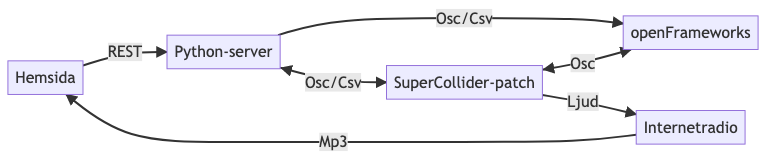
\includegraphics[width=0.5\textwidth]{../media/flowchart.png}
% \caption{Översiktsdiagram av system}
% \end{figure}

\begin{figure*}
\centering
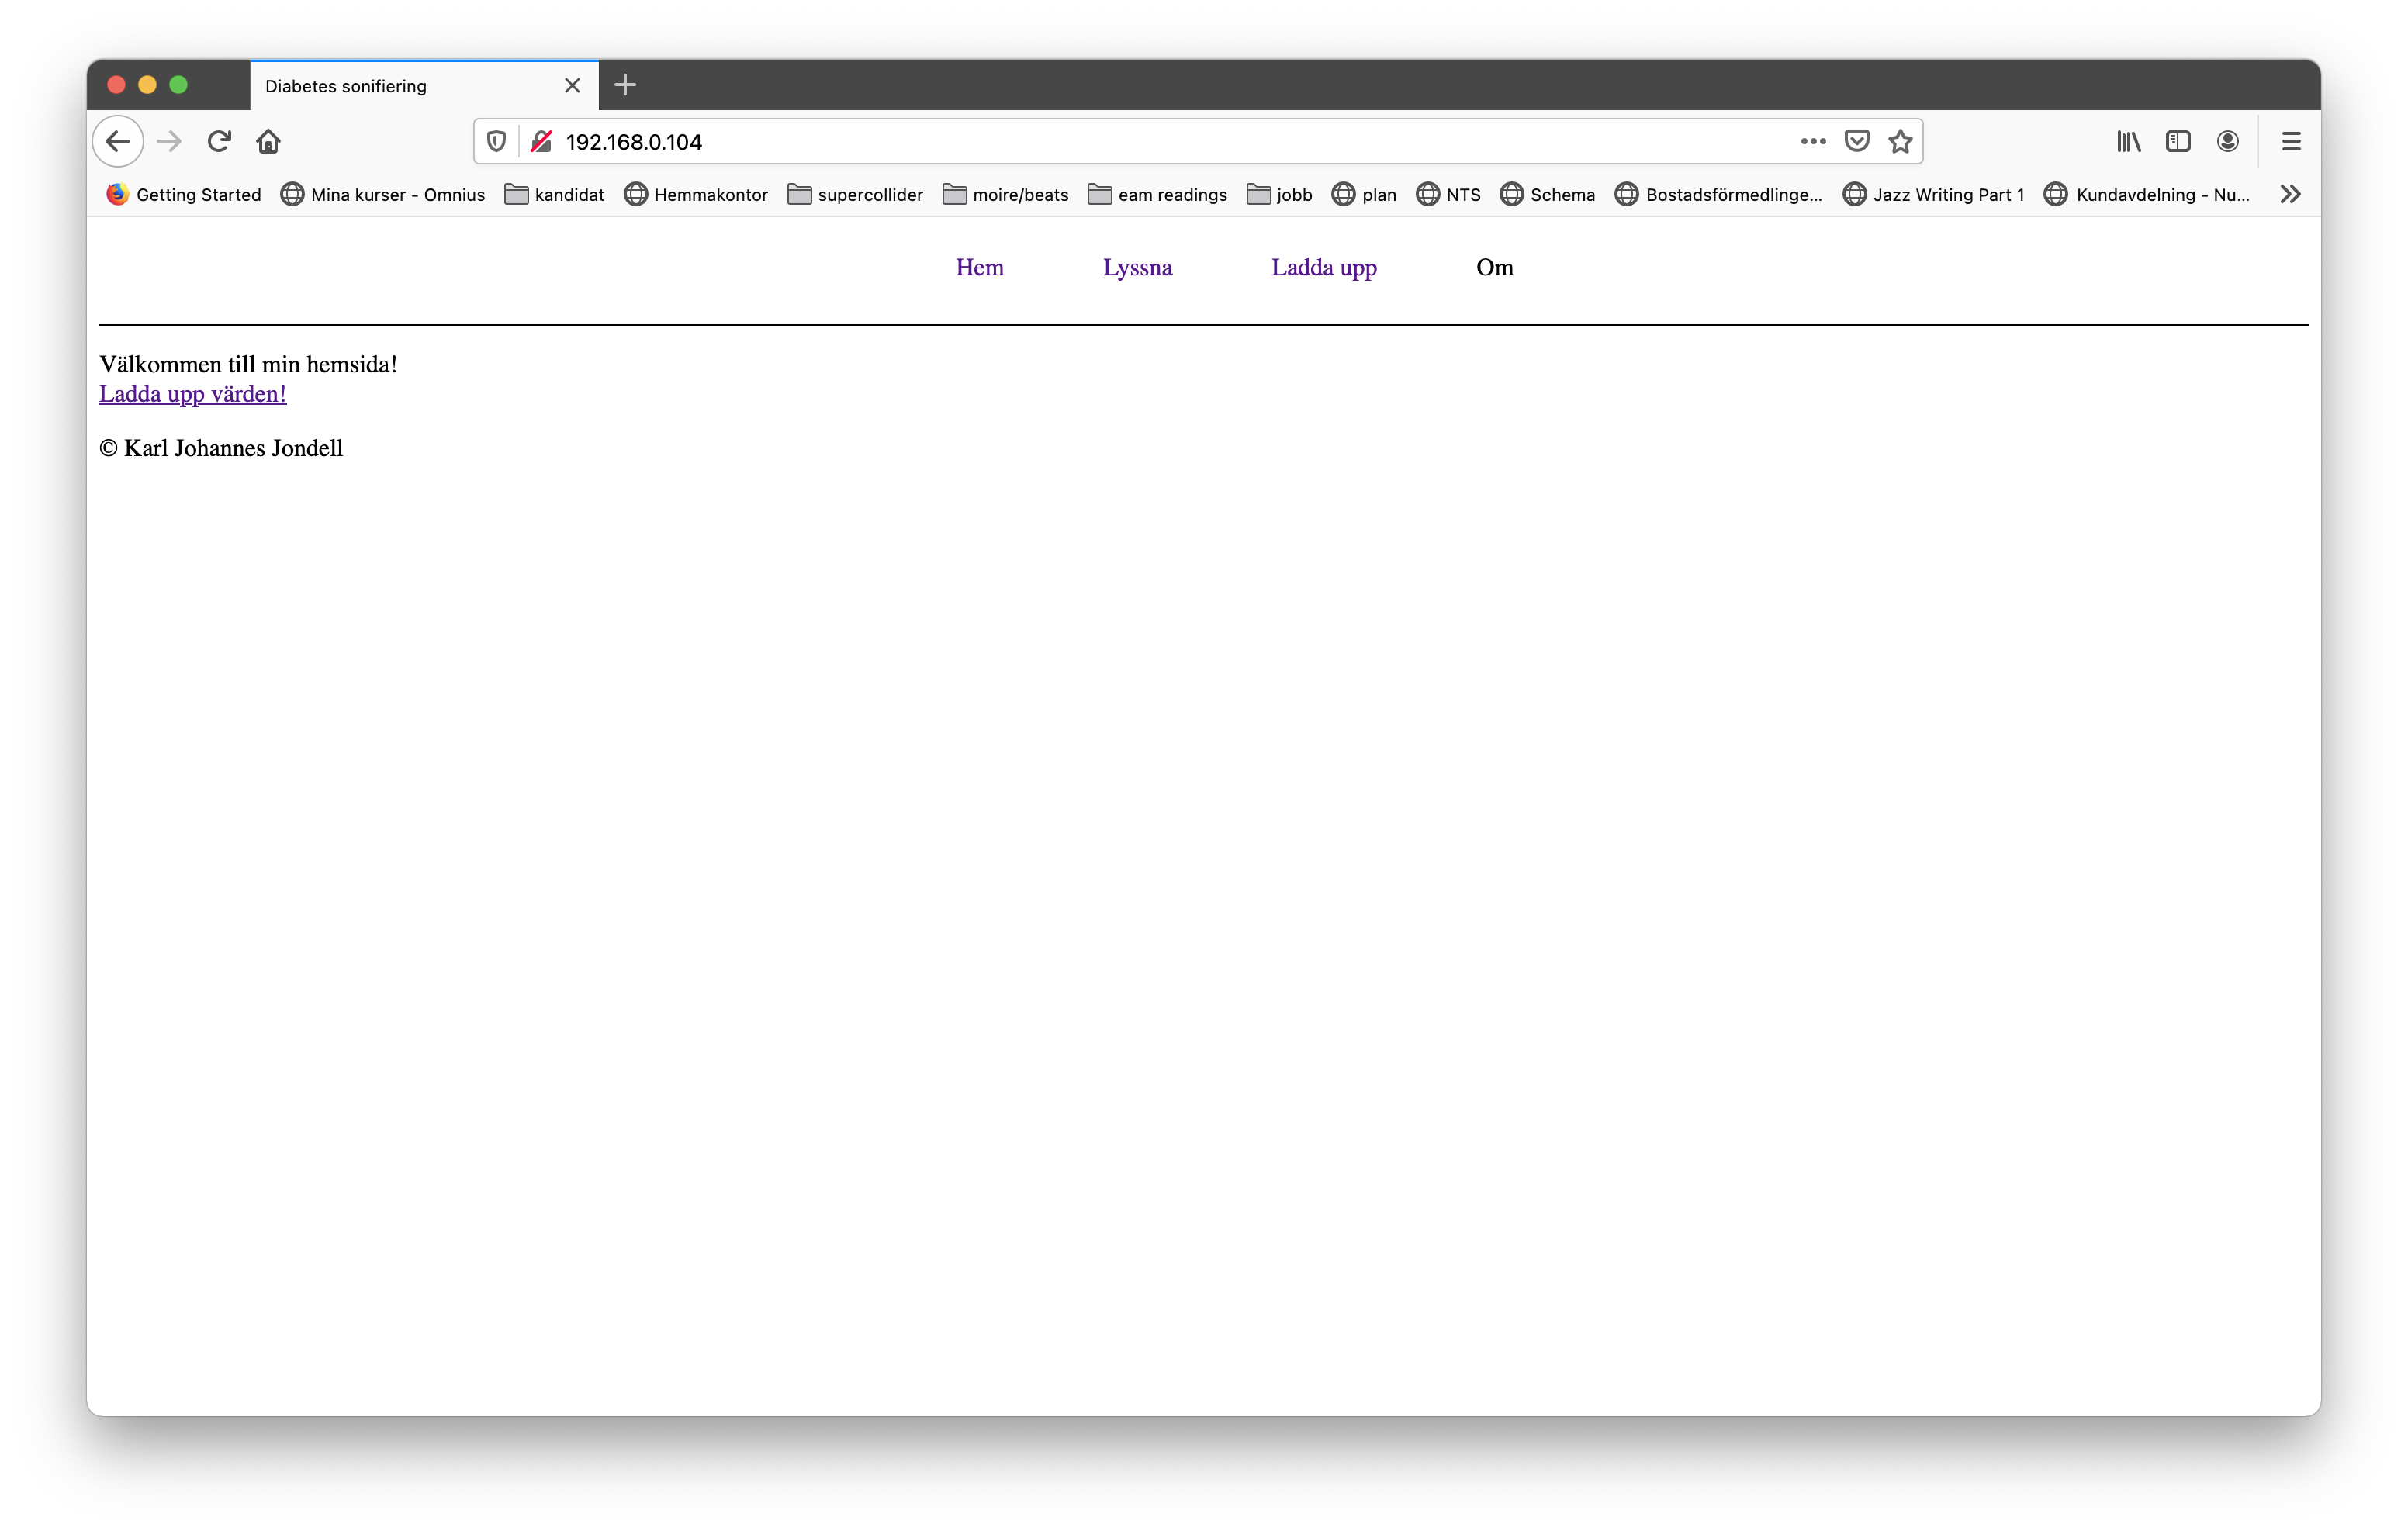
\includegraphics[width=\textwidth]{../media/hemsida.png}
\caption{Skärmdump av hemsida (\emph{temporär})}
\label{hemsida}
\end{figure*}

\subsection*{SuperCollider-system}
\addcontentsline{toc}{subsection}{SuperCollider-system}
% TODO LÄGG TILL ETT BLOCKDIAGRAM SOM ILLUSTRERAR SUPERCOLLIDER SYSTEMET
I SuperCollider-programmet representeras varje instans av mätdata av ett \emph{objekt}, som innehåller attribut som bland annat: register, skala, speltid, klangkälla/\emph{SynthDef}, tillhörande \emph{Pattern} och musikalisk funktion. Programmet innehåller också en funktion som behandlar inkommande OSC-meddelanden från Python-servern.

%Varje instans av mätdata existerar som ett \emph{objekt} (motsvarande en ljudkälla, inte schaefferiansk) i musiken, objekten har vissa attribut (såsom register, spatiell kodning, etc). 

\subsubsection*{Kösystem}
\addcontentsline{toc}{subsubsection}{\emph{Kösystem}}
När en deltagare laddar upp sina värden på webbplatsen   

\subsection*{Webbplats}
\addcontentsline{toc}{subsection}{Webbplats}
Webbplats består av en s.k. \emph{frontend} och en \emph{backend}
\subsubsection*{Frontend}
\addcontentsline{toc}{subsubsection}{\emph{Frontend}}
1. beskriv vad frontend är för något
2. beskriv tekniken (react.js)

\subsubsection*{Backend}
\addcontentsline{toc}{subsubsection}{\emph{Backend}}
1. beskriv vad backend är för något (API?)
2. flask, darkice/icecast också kanske? 


\section*{Musiken}
\addcontentsline{toc}{section}{Musiken}

% Lager, eller vilka SynthDefar jag har:
% 1. GSM (drone, eller bas/fundament, eller pad...)
% 2. Sinusvågor och elektroniska störningsljud (arpeggio, rytmiska, sextondelar, tempo)
% 3. Wavetable (pad)
% 4. JLC bas? resonator hum ? andra ljud ? ?? ? ? 

De musikaliska funktioner jag har representerade är dels ett fundament eller grund som utgörs av ett 

%Den konstnärliga friheten. Hur pass mycket kontroll som överlåtes till \enquote{serien} (i detta fall blodsockervärdet). Behöver musiken gestalta, spegla, estetisera erfarenheten som diabetiker? Eller vara intresseväckande, tillgänglig, \enquote{relaterbar}? 

\subsection*{Rumslighet}
\addcontentsline{toc}{subsection}{Rumslighet}
En \enquote{kör} av blodsockervärden, spatialiserade i nån mening för att ge en känsla av påverkan eller åverkan på musiken. 

Konsertupplevelse (i Lilla salen? spela ett utdrag ur liveströmmen...)

\subsection*{Temporalitet}
\addcontentsline{toc}{subsection}{Temporalitet}
Den tidsmässiga uppfattningen av musiken. En 24/7 livestream av musiken (hur utgörs lyssnadet? formen? \emph{Slow as possible}, \emph{Longplayer} och liknande...)

\subsection*{Generativt}
\addcontentsline{toc}{subsection}{Generativt}
Musiken är generativ. Serialism?

\section*{Sammanfattning}
\addcontentsline{toc}{section}{Sammanfattning}
Lärdomar etc...

\end{multicols}

\twocolumn

\printbibliography[type=book,title={Böcker}]
\printbibliography[type=article,title={Artiklar}]

\end{document}

